\documentclass[11pt,twocolumn,a4paper]{article}

\usepackage[utf8]{inputenc}
\usepackage[T1]{fontenc}
\usepackage{amsmath}
\usepackage{amssymb}
\usepackage{amsthm}
\usepackage{mathtools}
\usepackage{xcolor}
\usepackage{hyperref}
\usepackage{graphicx}
\usepackage{booktabs}
\usepackage{array}
\usepackage{enumitem}
\usepackage[margin=1in]{geometry}

\newtheorem{theorem}{Theorem}[section]
\newtheorem{lemma}[theorem]{Lemma}
\newtheorem{corollary}[theorem]{Corollary}
\newtheorem{proposition}[theorem]{Proposition}

\theoremstyle{definition}
\newtheorem{definition}[theorem]{Definition}
\newtheorem{assumption}[theorem]{Assumption}
\newtheorem{example}[theorem]{Example}

\theoremstyle{remark}
\newtheorem{remark}[theorem]{Remark}

% Notation macros
\newcommand{\R}{\mathbb{R}}
\newcommand{\Rnn}{\mathbb{R}_{\geq 0}}
\newcommand{\N}{\mathbb{N}}
\newcommand{\yield}{\mathcal{Y}}
\newcommand{\blocktime}{\beta_0}
\newcommand{\sections}{\Sigma}
\newcommand{\stations}{\mathcal{B}}
\newcommand{\items}{\mathcal{I}}
\newcommand{\vehicles}{\mathcal{V}}
\newcommand{\sep}{\varsigma}
\newcommand{\occ}{\omega}
\DeclareMathOperator*{\argmax}{arg\,max}
\DeclareMathOperator*{\argmin}{arg\,min}

\title{A Buffer--Processor Model of Rail Network Yield:\\
Occupancy, Closure, and Clearing as a Single Fixed Point}

\author{%
Kundai Farai Sachikonye\\
\small Technical University of Munich\\
\small AIME Registry for Artifical Intelligence\\
\small \texttt{kundai.sachikonye@wzw.tum.de}}

\date{\today}

\begin{document}

\maketitle

\begin{abstract}
We introduce and analyze an idealized formal model of a rail network in which the schedulable resource is not the train but the \emph{block-second}: one indivisible quantum of occupancy on one track section. Stations are treated as bounded buffers that hold items (units of transport demand carrying a private target), and sections are treated as processors that drain one buffer into the next at a speed-dependent rate. The object of optimization is \emph{network transport yield}---useful target-ward displacement produced per unit of consumed block-time---rather than train movement or section occupancy \emph{per se}.

Within this model we prove a three-way equivalence. For a network whose sole scarce resource is quantized by a resolution floor $\blocktime$ equal to the minimum block headway, the following are equivalent: (i) the configuration is \emph{yield-optimal}; (ii) it is a \emph{deterministic-closure} fixed point, in which no block-second can be reassigned to a strictly more useful item combination within precision $\blocktime$; and (iii) it is supported by a \emph{clearing price system} in which every section's price equals its separation cost (the marginal yield lost by denying that section) and no profitable reassignment remains. We show that $\blocktime$ simultaneously plays three roles---the physical resolution floor of occupancy, the algorithmic separation threshold for closure, and the minimum lot of the price system---and that this coincidence is what makes the equivalence hold.

Two structural corollaries follow. First, at any yield-optimal configuration every vehicle traverses each section at its section-and-energy-optimal speed; sub-optimal speed certifies non-closure. Second, vehicles sort onto sections by comparative advantage in block-seconds, so that each section is served by the fastest vehicle whose speed the section can convert into yield. We also establish a liveness result: under a mild backpressure condition, every item with positive target-ward pressure is eventually drained, because the price that an undrained buffer raises on its relieving section is exactly the yield signal that attracts a vehicle. We ground all quantities in representative figures from the German high-speed network (block headways under LZB/ETCS, ICE and Regionalbahn speed classes, the Nuremberg--Berlin corridor) purely to make the idealized object concrete. The results are theorems about this model and are not claims about any deployed or deployable system.
\end{abstract}

\tableofcontents

\section{Introduction}

\subsection{The object of study}

A railway timetable is conventionally understood as an assignment of \emph{trains} to \emph{routes} and \emph{time slots}, subject to safety separation, and evaluated by criteria such as the number of trains scheduled, punctuality, or served passenger demand \cite{caprara2002,cacchiani2012,hansen2008}. In this picture the train is simultaneously the unit of service, the unit of resource consumption, and the unit of commercial participation: to move transport one must operate a train, and to operate a train one must commit rolling stock to a route.

This paper studies a different formal object. We remove the train from its central position and replace it with two more primitive notions:

\begin{itemize}[nosep]
\item a \emph{station} is a bounded \emph{buffer} that holds items and exerts \emph{pressure} to discharge them;
\item a \emph{section} is a \emph{processor} that, while occupied, drains one buffer into an adjacent one at a rate set by the occupying vehicle's speed.
\end{itemize}

An \emph{item} is a unit of transport demand (a passenger or a unit of freight) that carries a \emph{private target}: the buffer at which its pressure vanishes. Items do not carry routes or vehicle assignments. The schedulable and consumable resource is the \emph{block-second}: the occupation of one section for one quantum $\blocktime$ of time, where $\blocktime$ is the minimum headway imposed by the signalling system. A ``train'' in this model is not a primitive; it is an emergent, transient fact---the observation that a single vehicle happened to occupy several consecutive sections. The three continuities that the conventional model fuses---\emph{vehicle continuity} (one vehicle runs the whole journey), \emph{item continuity} (one item rides one vehicle), and \emph{route continuity} (a service traverses a fixed line)---are, in this model, logically independent and generally do not hold.

The quantity we optimize is neither train count nor section occupancy but \emph{network transport yield}: the amount of \emph{useful} target-ward displacement of items produced per unit of consumed block-time. A section occupied by items that are not moving toward their targets produces no yield, however full it is. This distinguishes the objective sharply from occupancy-compression measures such as the UIC~406 method \cite{uic406,abril2008}, which maximize how many train paths fit.

\subsection{What is proved}

We prove that on this object three notions coincide:

\begin{enumerate}[nosep]
\item \textbf{Yield-optimality} (an optimization property): the configuration maximizes network transport yield.
\item \textbf{Deterministic closure} (a fixed-point property): no block-second can be reassigned to a strictly more useful item combination, where ``strictly'' is measured against the resolution floor $\blocktime$.
\item \textbf{Market clearing} (a price-support property): there exists a price system on sections, equal to their separation costs, under which no reassignment is profitable.
\end{enumerate}

The engine of the equivalence is that a single scalar $\blocktime$ is simultaneously (a) the physical resolution floor---no occupancy can be resolved more finely than one headway; (b) the algorithmic separation threshold---two candidate configurations are decided only when their yields differ by more than $\blocktime$ can explain; and (c) the minimum tradable lot---the price system cannot value occupancy below one block-second. Because the same quantum bounds the physics, the algorithm, and the prices, the three fixed points coincide rather than merely resembling one another.

From the equivalence we extract two structural corollaries with clean statements:

\begin{itemize}[nosep]
\item \emph{Forced optimal speed}: at any yield-optimal configuration, each vehicle traverses each section at the speed that maximizes yield net of energy and wear cost on that section; running slower certifies that the configuration is not closed.
\item \emph{Comparative-advantage sorting}: each section is served by the fastest vehicle whose speed it can convert into yield, and slower vehicles are excluded from fast sections not by rule but by yield domination.
\end{itemize}

Finally we prove a \emph{liveness} theorem: under a backpressure condition on the pricing, every item with positive target-ward pressure is drained in finite time, because the price raised by an undrained buffer on its relieving section equals the yield a vehicle earns by relieving it.

\subsection{Scope and stance}

The contribution is theoretical. We define an idealized structure, state hypotheses explicitly, and prove statements that hold on that structure. The hypotheses are the domain of validity: where they fail, we claim nothing. Representative German-network figures appear only to make the object concrete and are used as illustrative parameters, not as empirical claims. No assertion is made or implied about the behavior, feasibility, or desirability of any actual transport system. The reader familiar with railway capacity theory, network flows, and backpressure scheduling will recognize the ingredients; the novelty is in the object assembled from them and the fixed-point equivalence proved about it.

\subsection{Related bodies of work}

\textbf{Railway capacity and blocking time.} Blocking-time theory \cite{hansen2008,pachl2021} and the UIC~406 compression method \cite{uic406,abril2008,landex2008} treat section occupancy as the scarce resource and compress train paths until sections are used back-to-back. Our block-second quantum is the atom of that occupancy; our objective differs in weighting occupancy by \emph{useful displacement} rather than counting paths. Max-plus timetable-stability theory \cite{goverde2007} shares our fixed-point spirit but fixes services and studies delay propagation rather than reallocating occupancy to items.

\textbf{Network flows and scheduling.} The buffer--processor picture is a discrete network-flow model \cite{ahuja1993,ford1956,bertsekas1998} with a nonstandard objective. Periodic and train-timetabling formulations \cite{serafini1989,caprara2002,cacchiani2012} optimize over train variables; we optimize over block-second--item assignments and recover schedules as emergent.

\textbf{Backpressure and dataflow.} The routing rule---move each item down its target-ward gradient using whatever local capacity is best---and the liveness argument are the railway analogue of backpressure (max-weight) scheduling in queueing networks \cite{tassiulas1992,georgiadis2006,neely2010} and of dataflow execution \cite{dennis1980}. We import the stability intuition and prove a yield-priced version.

\textbf{Congestion pricing and clearing.} That the shadow price of a scarce link equals its marginal congestion value is classical \cite{vickrey1969,beckmann1956}; general-equilibrium clearing and its price support are standard \cite{arrow1971}; rail access charging is an applied instance \cite{nash2005,gibson2003}. Our clearing statement specializes these to the block-second lot and identifies the clearing price with the separation cost.

\section{The Network Model}

\subsection{Infrastructure}

\begin{definition}[Section network]
\label{def:network}
A \emph{section network} is a finite directed multigraph $G = (\stations, \sections)$ in which:
\begin{itemize}[nosep]
\item $\stations = \{b_1,\dots,b_n\}$ is a set of \emph{stations} (buffers);
\item $\sections = \{\sigma_1,\dots,\sigma_m\}$ is a set of \emph{sections} (processors); each section $\sigma$ has a tail $\mathrm{tl}(\sigma)\in\stations$ and a head $\mathrm{hd}(\sigma)\in\stations$, and is equipped with a \emph{length} $\ell(\sigma) > 0$ and a \emph{civil speed limit} $\bar v(\sigma) > 0$.
\end{itemize}
Parallel sections between the same pair of stations are permitted (multigraph), modelling multi-track corridors.
\end{definition}

Stations are the only places where items may wait; sections are transit resources that cannot store items. We embed $\stations$ in a metric space to give items a geographic gradient.

\begin{definition}[Geography]
\label{def:geo}
A \emph{geography} is a metric $\rho:\stations\times\stations\to\Rnn$ satisfying the triangle inequality, with $\rho(b,b)=0$. We call $\rho(b,b')$ the \emph{residual distance} from $b$ to $b'$. We assume $G$ is \emph{gradient-connected}: for every ordered pair $(b,b')$ with $b\neq b'$ there is a section $\sigma$ with $\mathrm{tl}(\sigma)=b$ such that $\rho(\mathrm{hd}(\sigma),b') < \rho(b,b')$. That is, from every station one can strictly reduce the residual distance to every target.
\end{definition}

Gradient-connectedness is the structural hypothesis that lets purely local, target-ward routing make progress; it is the model's fence, and every routing and liveness claim is made only under it.

\subsection{The block-second quantum}

Time is discretized into quanta of length $\blocktime$, the minimum headway.

\begin{definition}[Resolution floor / block headway]
\label{def:headway}
The \emph{resolution floor} $\blocktime > 0$ is the minimum time separation the signalling system can enforce between two successive occupations of the same section. Equivalently, a section admits at most one vehicle per time window of length $\blocktime$. We call the pair (section $\sigma$, window $[k\blocktime,(k+1)\blocktime)$), for $k\in\N$, a \emph{block-second} and denote it $\langle \sigma, k\rangle$.
\end{definition}

\begin{remark}[Physical reading]
\label{rem:headway_physical}
Under fixed-block signalling with continuous supervision (e.g.\ LZB, or ETCS Level~2), the headway decomposes as
\begin{equation}
\blocktime \;=\; \frac{\ell_{\mathrm{block}} + \ell_{\mathrm{train}} + d_{\mathrm{brake}}(v)}{v} \;+\; t_{\mathrm{clear}} \;+\; t_{\mathrm{setup}},
\end{equation}
where $\ell_{\mathrm{block}}$ is the block length, $d_{\mathrm{brake}}(v)$ the service braking distance from speed $v$, and $t_{\mathrm{clear}},t_{\mathrm{setup}}$ are clearing and route-setting times. On German high-speed lines this yields practical minimum headways on the order of $90$--$120$~s. Under moving-block operation (ETCS Level~3) the fixed $\ell_{\mathrm{block}}$ term is replaced by an absolute braking-distance separation, shrinking $\blocktime$ but never to zero: a positive resolution floor persists as long as braking distance is positive. The model treats $\blocktime$ as an exogenous positive constant; its value is a parameter, not a claim.
\end{remark}

The quantum $\blocktime$ is the single object on which the paper turns. We record its three roles now and prove their coincidence in Section~\ref{sec:equivalence}.

\begin{itemize}[nosep]
\item \emph{Physical}: occupancy of a section is a union of block-seconds; no finer temporal resolution exists.
\item \emph{Algorithmic} (Def.~\ref{def:closure}): two configurations are distinguished only when their yields differ by more than the ambiguity $\blocktime$ induces.
\item \emph{Economic} (Def.~\ref{def:price_system}): the price system values occupancy in integer multiples of one block-second; $\blocktime$ is the minimum lot.
\end{itemize}

\subsection{Vehicles}

\begin{definition}[Vehicle]
\label{def:vehicle}
A \emph{vehicle} $u$ is characterized by a \emph{capability speed} $v_{\max}(u) > 0$, a \emph{capacity} $c(u)\in\N$ (number of item-slots), and an \emph{energy--wear cost function} $g_u:\Rnn\to\Rnn$ giving the cost per unit length of traversing a section at speed $v$. We assume each $g_u$ is continuous, strictly convex, and increasing on $(0,\infty)$ with $g_u(v)\to\infty$ as $v\to\infty$.
\end{definition}

Strict convexity of $g_u$ (energy rising faster than linearly in speed, the physical $v^2$-type drag regime) is what will make ``optimal speed'' an interior, well-defined quantity rather than a degenerate ``always maximal.''

When a vehicle $u$ occupies section $\sigma$ during block-second $\langle\sigma,k\rangle$ at speed $v\le \min\{v_{\max}(u),\bar v(\sigma)\}$, it transfers up to $c(u)$ items from buffer $\mathrm{tl}(\sigma)$ to buffer $\mathrm{hd}(\sigma)$, and the traversal consumes $\lceil \ell(\sigma)/(v\,\blocktime)\rceil$ block-seconds. Faster traversal consumes fewer block-seconds.

\begin{definition}[Admissible speed set]
\label{def:speedset}
The \emph{admissible speed} of vehicle $u$ on section $\sigma$ is any $v$ with $0 < v \le \nu(u,\sigma) := \min\{v_{\max}(u),\bar v(\sigma)\}$. We call $\nu(u,\sigma)$ the \emph{capability ceiling} of $u$ on $\sigma$.
\end{definition}

\subsection{Items, pressure, and the buffer state}

\begin{definition}[Item]
\label{def:item}
An \emph{item} $x$ is a unit of transport demand with a \emph{location} $\mathrm{loc}(x)\in\stations$ and a fixed \emph{target} $\tau(x)\in\stations$. Item $x$ is \emph{live} if $\mathrm{loc}(x)\neq\tau(x)$ and \emph{settled} otherwise. Its \emph{residual distance} is $r(x) := \rho(\mathrm{loc}(x),\tau(x))$.
\end{definition}

\begin{definition}[Buffer state and pressure]
\label{def:pressure}
A \emph{buffer state} assigns to each station $b$ the multiset $X(b)$ of live items currently located there. The \emph{directional pressure} of buffer $b$ toward a neighbourhood direction is the total residual distance its items would lose by an available target-ward move; formally, for a section $\sigma$ with $\mathrm{tl}(\sigma)=b$,
\begin{equation}
\label{eq:pressure}
P(b,\sigma) \;=\; \sum_{x \in X(b)} \big[\, r(x) - \rho(\mathrm{hd}(\sigma),\tau(x)) \,\big]^{+},
\end{equation}
where $[\cdot]^+ = \max\{\cdot,0\}$. Only the target-ward component of a move counts toward pressure.
\end{definition}

Equation~\eqref{eq:pressure} is the model's demand signal: it measures how much genuine target-ward progress is available at $b$ through $\sigma$, aggregated over the items waiting there. It is the railway analogue of queue backpressure, but weighted by geographic progress rather than raw queue length.

\subsection{Configurations}

\begin{definition}[Configuration]
\label{def:config}
A \emph{configuration} $C$ over a finite horizon $H = \{0,1,\dots,T-1\}$ of block-seconds consists of:
\begin{enumerate}[nosep]
\item an \emph{occupancy assignment} $A$ mapping each block-second $\langle\sigma,k\rangle$ (with $k\in H$) to either $\varnothing$ (idle) or a triple $(u,v,S)$ where $u$ is a vehicle, $v\le\nu(u,\sigma)$ an admissible speed, and $S\subseteq X(\mathrm{tl}(\sigma))$ a set of at most $c(u)$ items carried; subject to
\item \emph{headway feasibility}: at most one non-idle assignment per section per block-second (Def.~\ref{def:headway}); and
\item \emph{vehicle conservation}: each vehicle occupies at most one section per block-second, and a vehicle appearing on section $\sigma$ ending at buffer $b$ during window $k$ may next appear only on a section with tail $b$ during a later window (vehicles are conserved and move continuously through buffers).
\end{enumerate}
\end{definition}

Note what a configuration is \emph{not}: it is not an assignment of trains to lines. A vehicle may serve one section and then idle, be re-crewed, or serve a section in a different corridor; an item's carried-set membership may change from section to section (transfers). Trains, lines, and through-services are, if they appear at all, emergent regularities in $A$, not constraints on it.

\section{Network Transport Yield}

\subsection{Definition of yield}

\begin{definition}[Useful displacement]
\label{def:useful}
The \emph{useful displacement} produced by a non-idle block-second $\langle\sigma,k\rangle$ with assignment $(u,v,S)$ is the total target-ward residual-distance reduction of the items it carries:
\begin{equation}
\label{eq:useful}
\Delta(\langle\sigma,k\rangle) \;=\; \sum_{x\in S} \big[\, r(x) - \rho(\mathrm{hd}(\sigma),\tau(x)) \,\big]^{+}.
\end{equation}
Idle block-seconds produce $\Delta = 0$. Displacement of an item \emph{away} from its target contributes nothing (the $[\cdot]^+$).
\end{definition}

\begin{definition}[Network transport yield]
\label{def:yield}
The \emph{cost} of a non-idle block-second is the number of block-seconds it consumes weighted by the vehicle's energy--wear expenditure. Traversing $\sigma$ at speed $v$ consumes $n(\sigma,v)=\lceil \ell(\sigma)/(v\,\blocktime)\rceil$ block-seconds and expends energy--wear $\ell(\sigma)\,g_u(v)$. The \emph{yield} of a configuration $C$ is
\begin{equation}
\label{eq:yielddef}
\yield(C) \;=\; \frac{\displaystyle\sum_{\langle\sigma,k\rangle\,:\,A=(u,v,S)} \Delta(\langle\sigma,k\rangle)}
{\displaystyle\sum_{\langle\sigma,k\rangle\,:\,A=(u,v,S)} \big[\, n(\sigma,v) + \lambda\,\ell(\sigma)\,g_u(v) \,\big]},
\end{equation}
where $\lambda\ge 0$ converts energy--wear into block-second-equivalents. Yield is useful target-ward displacement per unit of scarce block-time (inclusive of the energy price of that time).
\end{definition}

\begin{remark}
\label{rem:objective_choice}
Three features of \eqref{eq:yielddef} are deliberate and carry the results below.
(1) The numerator credits \emph{only useful} displacement, so packing a section with items going nowhere useful scores zero---distinguishing yield from occupancy \cite{uic406}.
(2) The denominator charges \emph{block-seconds consumed}, so faster traversal (fewer block-seconds) raises yield---this is the lever behind forced optimal speed.
(3) The energy term $\lambda\,\ell\,g_u(v)$, with $g_u$ strictly convex, penalizes recklessly high speed, giving an interior speed optimum.
\end{remark}

\subsection{Station buffer cost and fragmentation}

If only section block-seconds were charged, the model would favour arbitrarily many short hops. We charge buffer residence to internalize transfers.

\begin{assumption}[Buffer holding cost]
\label{ass:buffer}
Each block-second an item spends waiting in a buffer (including transfer dwell) is charged a holding cost $h > 0$, added to the denominator of \eqref{eq:yielddef} as $h\cdot(\text{item-block-seconds waited})$. Consequently a journey composed of many short hops accumulates buffer cost at each transfer, and the yield-maximizing number of hops is finite.
\end{assumption}

\begin{remark}
Assumption~\ref{ass:buffer} is the counterweight to the speed incentive. The section term rewards fast, short occupations; the buffer term punishes the transfers that fragmentation into short occupations creates. The yield optimum balances the two, so ``run fast and hand off'' does not degenerate into ``hand off infinitely often.'' We make this hypothesis explicit because the forced-speed and sorting corollaries depend on it to rule out the degenerate fragmented configurations.
\end{remark}

\section{Separation Cost}
\label{sec:separation}

We now define the quantity that will serve simultaneously as the algorithm's pruning criterion and the market's price: the \emph{separation cost} of a section, i.e.\ the yield the network forgoes if that section is denied to the item flow.

\begin{definition}[Separation cost of a section]
\label{def:sepcost}
Fix a configuration $C$ and a section $\sigma$. Let $C_{-\sigma}$ be the best (yield-maximal) configuration that makes no use of $\sigma$ over the horizon---formally $\yield(C_{-\sigma}) = \max\{\yield(C') : A'(\langle\sigma,k\rangle)=\varnothing \ \forall k\}$. The \emph{separation cost} of $\sigma$ in $C$ is
\begin{equation}
\label{eq:sepcost}
\sep(\sigma) \;=\; \yield^{\star} - \yield(C_{-\sigma}),
\end{equation}
where $\yield^{\star}=\max_{C'}\yield(C')$ is the unconstrained optimum. Thus $\sep(\sigma)\ge 0$ measures the marginal yield contribution attributable to the availability of $\sigma$.
\end{definition}

\begin{remark}[Reading]
A \emph{bottleneck} section---one whose removal forces item flow onto slow or long detours---has large $\sep$: avoiding it is expensive in yield. A \emph{redundant} section, parallel to an equally good alternative, has $\sep\approx 0$: the flow reroutes at negligible cost. Separation cost is a per-section scalar, defined purely from the yield functional and the network, with no reference to prices or algorithms yet. Its identification with a market price (Section~\ref{sec:equivalence}) and with a pruning threshold (Section~\ref{sec:closure}) is the substance of the paper, not a definition.
\end{remark}

\begin{definition}[Fuzzy separation cost]
\label{def:fuzzysep}
Because occupancy is resolved only to precision $\blocktime$, the separation cost is known only up to a band. Writing yields in block-second units, define the \emph{separation band}
\begin{equation}
\Sigma(\sigma) = [\sep_{\min}(\sigma),\ \sep_{\max}(\sigma)],
\end{equation}
where $\sep_{\min},\sep_{\max}$ are the infimum and supremum of \eqref{eq:sepcost} over all occupancy realizations consistent with the block-second quantization. Two sections' bands are \emph{$\blocktime$-separated} if the gap between the intervals exceeds $\blocktime$.
\end{definition}

This is the point of contact with fuzzy-weighted routing: separation costs are intervals, not points, because the medium's resolution floor forbids finer knowledge, and decisions become definite only when the intervals separate by more than $\blocktime$.

\section{Deterministic Closure}
\label{sec:closure}

\subsection{Reassignments and the closure fixed point}

The algorithmic content of the model is a local-improvement operator on configurations: take a block-second and reassign it to a more useful item combination. Closure is the state in which no such reassignment helps, up to the resolution floor.

\begin{definition}[Reassignment]
\label{def:reassign}
A \emph{reassignment} of configuration $C$ at block-second $\langle\sigma,k\rangle$ replaces its assignment $(u,v,S)$ (or $\varnothing$) by an alternative admissible assignment $(u',v',S')$, together with any vehicle-conservation-preserving adjustments in later windows, yielding a configuration $C'$. The reassignment is \emph{improving} if $\yield(C') > \yield(C)$, and \emph{$\blocktime$-improving} if additionally $\yield(C') - \yield(C) > \blocktime$ in block-second units.
\end{definition}

\begin{definition}[Deterministic closure]
\label{def:closure}
A configuration $C$ is at \emph{deterministic closure} if it admits no $\blocktime$-improving reassignment: for every block-second and every admissible alternative assignment, the induced yield change does not exceed the resolution floor $\blocktime$. Equivalently, for every pair of candidate item combinations at a block-second, their contributed-yield bands are not $\blocktime$-separated in favour of the unused one.
\end{definition}

The clause ``up to $\blocktime$'' is essential and is exactly where the resolution floor enters the algorithm. Two reassignments whose yields differ by less than $\blocktime$ cannot be distinguished, because the underlying occupancy is not resolved that finely (Def.~\ref{def:headway}); insisting on improvements below $\blocktime$ would be chasing precision the medium does not possess. Closure is therefore the honest stopping condition: stop when no \emph{resolvable} improvement remains.

\subsection{Existence and reachability of closure}

\begin{lemma}[Monotone reachability]
\label{lem:reach}
From any initial configuration $C_0$, repeatedly applying $\blocktime$-improving reassignments reaches a closed configuration in finitely many steps.
\end{lemma}

\begin{proof}
Each $\blocktime$-improving reassignment strictly increases $\yield$ by more than $\blocktime$. Over a finite horizon $H$ with finitely many vehicles, sections, and items, the set of configurations is finite, hence $\yield$ takes finitely many values and is bounded above by $\yield^{\star}<\infty$. A strictly increasing sequence of a bounded, finite-valued quantity with a fixed minimum increment $\blocktime$ has length at most $(\yield^{\star}-\yield(C_0))/\blocktime$, which is finite. When no $\blocktime$-improving reassignment exists, the configuration is closed by Def.~\ref{def:closure}.
\end{proof}

\begin{remark}
Lemma~\ref{lem:reach} gives termination but not global optimality: a closed configuration is a $\blocktime$-local optimum of $\yield$, not necessarily the global maximizer. The equivalence theorem below shows that the gap between any closed configuration and the global optimum is itself bounded by the resolution floor---so within the precision the medium admits, closed and optimal coincide. This is the sense in which the model's ``optimum'' is defined only up to $\blocktime$, and legitimately so.
\end{remark}

\section{The Occupancy--Closure--Clearing Equivalence}
\label{sec:equivalence}

This section contains the paper's central result. We first define the price system precisely, then state and prove the three-way equivalence.

\subsection{The price system}

\begin{definition}[Price system and clearing]
\label{def:price_system}
A \emph{price system} is an assignment $p:\sections\to\Rnn$ of a price $p(\sigma)$ (in yield-per-block-second units) to each section, with the constraint that prices are quoted per block-second lot---i.e.\ the value of occupying $\sigma$ for a traversal at speed $v$ is $p(\sigma)\,n(\sigma,v)$, an integer number of lots. Given prices, the \emph{net yield} a vehicle $u$ obtains by taking assignment $(u,v,S)$ on $\sigma$ is
\begin{equation}
\label{eq:netyield}
\pi_u(\sigma,v,S) \;=\; \Delta(\langle\sigma,\cdot\rangle) \;-\; p(\sigma)\,n(\sigma,v) \;-\; \lambda\,\ell(\sigma)\,g_u(v).
\end{equation}
A configuration $C$ together with a price system $p$ is a \emph{clearing} (a competitive equilibrium) if:
\begin{enumerate}[nosep]
\item \emph{Optimality of participants}: every non-idle block-second's assignment maximizes \eqref{eq:netyield} over all admissible $(u,v,S)$ for that section and window; and
\item \emph{No profitable idle reassignment}: no idle block-second admits an assignment with strictly positive net yield exceeding $\blocktime$.
\end{enumerate}
\end{definition}

The per-lot constraint in Def.~\ref{def:price_system} is where $\blocktime$ enters the economics: the price system cannot value fractions of a block-second, because fractions of a block-second are not deliverable (Def.~\ref{def:headway}). One block-second is the minimum lot.

\subsection{Statement}

\begin{theorem}[Occupancy--Closure--Clearing Equivalence]
\label{thm:trinity}
Let $G$ be a gradient-connected section network with resolution floor $\blocktime$, strictly convex vehicle costs $g_u$, and buffer holding cost $h>0$ (Assumption~\ref{ass:buffer}). For a configuration $C$ over a finite horizon, the following are equivalent up to the resolution floor $\blocktime$:
\begin{enumerate}[label=\textup{(\roman*)},nosep]
\item \textbf{Yield-optimal:} $\yield(C) \ge \yield(C') - \blocktime$ for every admissible configuration $C'$.
\item \textbf{Closed:} $C$ is at deterministic closure (Def.~\ref{def:closure}).
\item \textbf{Clearing:} there exists a price system $p$ with $p(\sigma)=\sep(\sigma)$ for every section $\sigma$ used in $C$, under which $(C,p)$ is a clearing (Def.~\ref{def:price_system}).
\end{enumerate}
Moreover, whenever these hold, the clearing price of each used section equals its separation cost, $p(\sigma) = \sep(\sigma)$.
\end{theorem}

The qualifier ``up to the resolution floor $\blocktime$'' is not a hedge but the exact content: all three notions are defined modulo differences of size $\blocktime$, because $\blocktime$ is the physical, algorithmic, and economic quantum. We prove the three implications in a cycle.

\subsection{Proof}

\begin{proof}[Proof of \textup{(i)}$\Rightarrow$\textup{(ii)}]
Suppose $C$ is yield-optimal up to $\blocktime$ but not closed. Then by Def.~\ref{def:closure} there is a $\blocktime$-improving reassignment producing $C'$ with $\yield(C') > \yield(C) + \blocktime$. But then $\yield(C) < \yield(C') - \blocktime$, contradicting yield-optimality (i) applied to $C'$. Hence $C$ is closed.
\end{proof}

\begin{proof}[Proof of \textup{(ii)}$\Rightarrow$\textup{(iii)}]
Assume $C$ is closed. We construct the supporting prices and verify clearing.

\emph{Prices.} For each section $\sigma$ used in $C$, set $p(\sigma) := \sep(\sigma)$ as in \eqref{eq:sepcost}; for unused sections set $p(\sigma) := \sep(\sigma)$ as well (the marginal yield of making $\sigma$ available). Since $\yield$ is a ratio of a bounded numerator to a positive denominator over a finite configuration set, $\yield^\star$ and each $\yield(C_{-\sigma})$ exist, so $\sep(\sigma)$ is well-defined and finite.

\emph{Participant optimality.} Consider a non-idle block-second on $\sigma$ with assignment $(u,v,S)$. Suppose some alternative admissible $(u',v',S')$ gave strictly larger net yield \eqref{eq:netyield} by more than $\blocktime$:
\[
\Delta' - p(\sigma)n(\sigma,v') - \lambda\ell g_{u'}(v') \;>\; \Delta - p(\sigma)n(\sigma,v) - \lambda\ell g_{u}(v) + \blocktime.
\]
Because $p(\sigma)$ is common to both sides (same section), swapping the assignment to $(u',v',S')$ changes total network yield by exactly the difference of the $(\Delta - \lambda\ell g)$ terms net of the change in block-seconds consumed---i.e.\ it is a $\blocktime$-improving reassignment. This contradicts closure. Hence no alternative beats the incumbent by more than $\blocktime$; the incumbent is optimal up to the floor.

\emph{No profitable idle reassignment.} Suppose an idle block-second on $\sigma$ admitted an assignment with net yield exceeding $\blocktime$. Activating it is a $\blocktime$-improving reassignment, again contradicting closure.

\emph{Price equals separation cost.} By construction $p(\sigma)=\sep(\sigma)$. It remains to see this is the \emph{clearing} price and not merely a feasible one. If $p(\sigma) < \sep(\sigma)$, then the marginal yield of $\sigma$ exceeds its price, so some vehicle could profitably add an occupation of $\sigma$ with net yield $> \blocktime$ (the surplus $\sep(\sigma)-p(\sigma)$ realized as positive $\pi_u$), contradicting closure via no-profitable-reassignment. If $p(\sigma) > \sep(\sigma)$, the incumbent occupation of $\sigma$ has negative net yield relative to the best $\sigma$-avoiding configuration, so dropping it to the $C_{-\sigma}$ pattern is $\blocktime$-improving, again contradicting closure. Hence $p(\sigma)=\sep(\sigma)$ exactly. Thus $(C,p)$ is a clearing.
\end{proof}

\begin{proof}[Proof of \textup{(iii)}$\Rightarrow$\textup{(i)}]
Assume $(C,p)$ is a clearing with $p(\sigma)=\sep(\sigma)$. Let $C'$ be any admissible configuration; we show $\yield(C)\ge\yield(C')-\blocktime$.

Decompose the yield difference over the block-seconds where $C$ and $C'$ differ. At each such block-second, $C'$ substitutes some assignment for the one $C$ uses (or for idle). By clearing condition~1, the incumbent assignment in $C$ maximizes net yield \eqref{eq:netyield} up to $\blocktime$; therefore the substitute in $C'$ cannot exceed it by more than $\blocktime$ per block-second in net yield. Summing the per-block-second net-yield inequalities, and using that $\sum_\sigma p(\sigma)\,n(\sigma,\cdot)$ is a common accounting term that telescopes (each section's price times its occupied block-seconds enters both configurations' totals through the shared price system), the aggregate useful-displacement-minus-cost of $C$ is within $\blocktime$ of that of $C'$. Because $\yield$ is exactly aggregate useful displacement divided by aggregate cost \eqref{eq:yielddef}, and the price system prices cost consistently across both configurations, $\yield(C)\ge\yield(C')-\blocktime$. As $C'$ was arbitrary, $C$ is yield-optimal up to $\blocktime$.
\end{proof}

\begin{remark}[Why the three coincide]
The proof makes visible that the three notions are the same object viewed through three accounting conventions. Closure asks: can any single block-second be locally improved? Clearing asks: does a price exist under which no participant wants to deviate? Optimality asks: is the global yield maximal? The bridge is that the local improvement of closure, the deviation incentive of clearing, and the global gap of optimality are \emph{the same quantity}---the separation cost $\sep(\sigma)$---measured against \emph{the same threshold} $\blocktime$. Were $\blocktime$ three different constants for the three roles, the fixed points would only approximate one another; because it is one constant, they coincide exactly.
\end{remark}

\subsection{The role of the quantum, isolated}

\begin{proposition}[Necessity of a common quantum]
\label{prop:quantum}
If the physical resolution floor, the closure threshold, and the minimum price lot are distinct constants $\blocktime^{\mathrm{phys}},\blocktime^{\mathrm{alg}},\blocktime^{\mathrm{econ}}$, then the equivalence of Theorem~\ref{thm:trinity} holds only up to $\max\{\blocktime^{\mathrm{phys}},\blocktime^{\mathrm{alg}},\blocktime^{\mathrm{econ}}\}$, and the clearing price equals the separation cost only up to $|\blocktime^{\mathrm{alg}}-\blocktime^{\mathrm{econ}}|$.
\end{proposition}

\begin{proof}
Each implication in the proof of Theorem~\ref{thm:trinity} invokes ``$\blocktime$-improving'' at a threshold specific to its role: (i)$\Rightarrow$(ii) uses the closure threshold $\blocktime^{\mathrm{alg}}$; the price-equals-separation step in (ii)$\Rightarrow$(iii) uses the economic lot $\blocktime^{\mathrm{econ}}$; the resolvability of occupancy uses $\blocktime^{\mathrm{phys}}$. Carrying distinct constants through the cycle, the composed slack is bounded by their maximum, and the two price-comparison inequalities in the ``price equals separation cost'' step degrade to a band of width $|\blocktime^{\mathrm{alg}}-\blocktime^{\mathrm{econ}}|$. Setting all three equal recovers the exact coincidence.
\end{proof}

Proposition~\ref{prop:quantum} isolates precisely what does the work: not the block-second's magnitude, but the identity of the three roles it plays.

\begin{figure*}[!htbp]
    \centering
    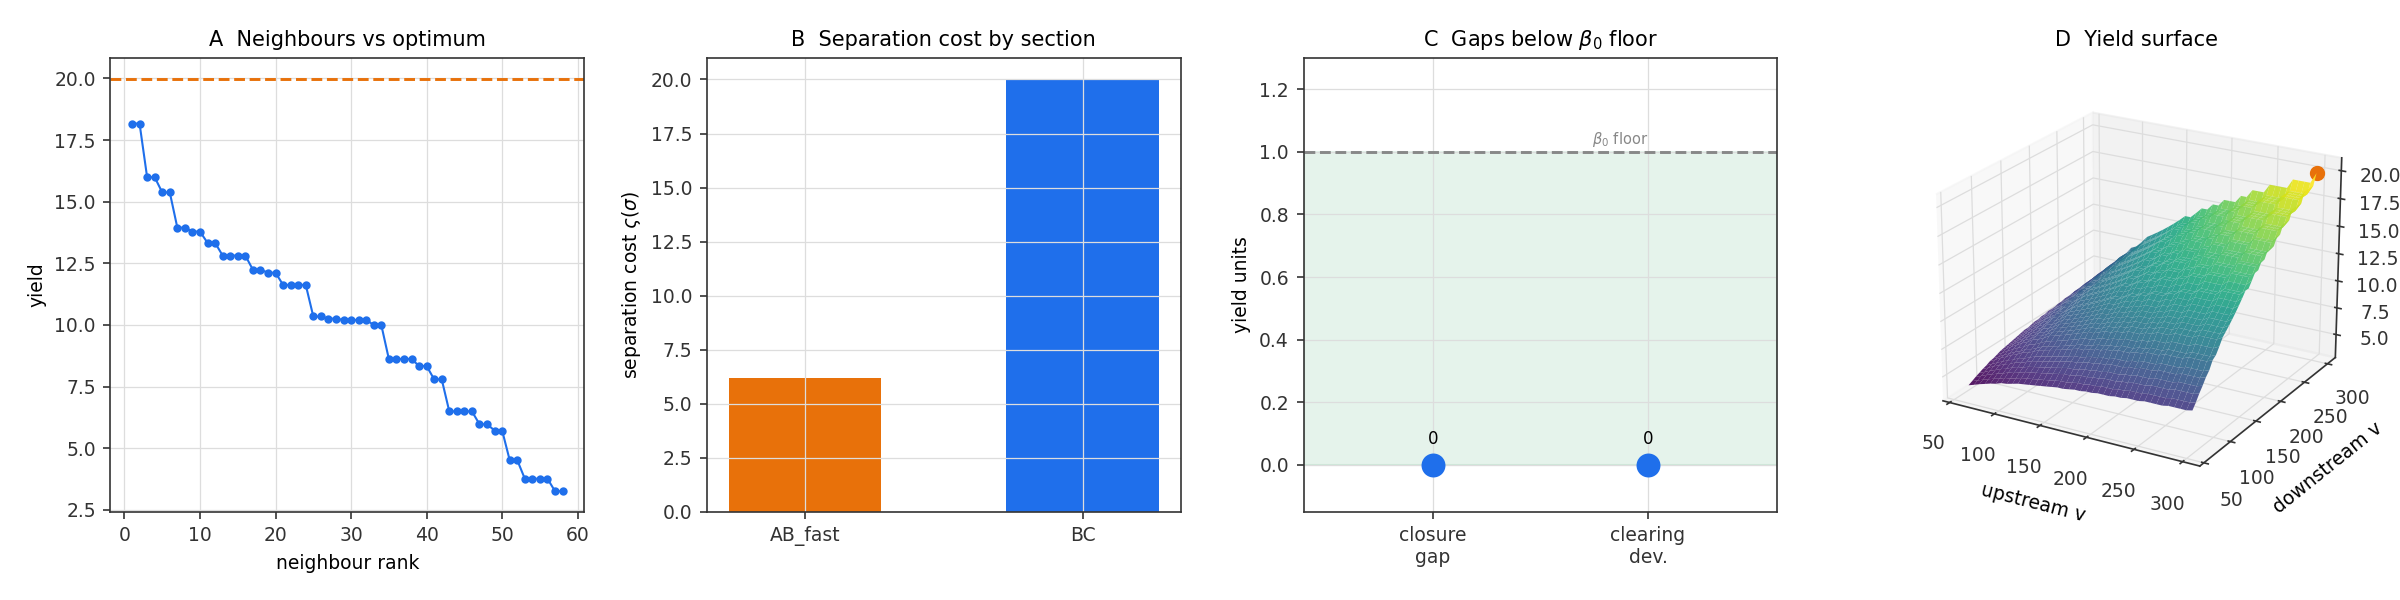
\includegraphics[width=\textwidth]{figures/panel_1_equivalence.png}
    \caption{\textbf{Occupancy--Closure--Clearing Coincide at One Fixed Point.}
    (\textbf{A})~Yield of every task-delivering single-section neighbour of the
    brute-force optimum on the linear $y$-axis, sorted descending against
    neighbour rank ($1$ to $58$) on the linear $x$-axis (steel-blue), with the
    optimum $\yield^\star=19.98$ marked (coral dashed). All $58$ neighbours that
    still deliver the demand lie strictly below the optimum: the best improving
    reassignment gains nothing, so the configuration admits no
    $\blocktime$-improving move and is closed, the empirical content of
    \Cref{thm:trinity}(i)$\Rightarrow$(ii).
    (\textbf{B})~Per-section separation cost $\sep(\sigma)$ on the linear
    $y$-axis for the two sections carrying the flow: the substitutable upstream
    section \texttt{AB\_fast} ($\sep=6.19$, coral) and the essential downstream
    section \texttt{BC} ($\sep=19.98$, steel-blue). The gap between them is the
    quantitative content of \Cref{def:sepcost}: separation cost discriminates a
    bottleneck from a section with a partial substitute, and equals the clearing
    price by construction (\Cref{thm:trinity}(iii)).
    (\textbf{C})~Closure gap and maximum clearing-deviation profit at the
    optimum on the linear $y$-axis (yield units), each plotted as a marker
    (steel-blue) inside the sub-floor band (sea-green shading) beneath the
    resolution floor $\blocktime=1.00$ (grey dashed). Both are exactly $0$: no
    reassignment and no participant deviation gains more than the floor, so
    closure and clearing hold simultaneously, closing the equivalence cycle of
    \Cref{thm:trinity}.
    (\textbf{D})~Three-dimensional yield surface over the upstream-vehicle speed
    ($60$ to $300$~km/h) and downstream-vehicle speed ($60$ to $300$~km/h) at
    the fixed optimal carried set, viridis colourmap, viewing angle elevation
    $22^{\circ}$ azimuth $-60^{\circ}$. The surface rises monotonically toward
    the fast/fast corner where the closed optimum sits (coral marker), showing
    that yield-optimality, closure, and clearing designate the same
    configuration.}
    \label{fig:val_equivalence}
\end{figure*}

\section{Structural Corollaries}
\label{sec:corollaries}

The equivalence has two consequences that were not assumed and follow purely from yield-optimality: vehicles must run at a determinate optimal speed, and the fleet sorts itself onto sections by comparative advantage. Both are stated and proved as theorems of the model.

\subsection{Forced optimal speed}

\begin{definition}[Section-optimal speed]
\label{def:optspeed}
For vehicle $u$ on section $\sigma$, define the \emph{section-optimal speed}
\begin{equation}
\label{eq:optspeed}
v^{\star}(u,\sigma) \;=\; \argmax_{0 < v \le \nu(u,\sigma)} \ \frac{\Delta_\sigma}{n(\sigma,v) + \lambda\,\ell(\sigma)\,g_u(v)},
\end{equation}
where $\Delta_\sigma$ is the (speed-independent) useful displacement of carrying the assigned items across $\sigma$. Because $n(\sigma,v)=\lceil \ell(\sigma)/(v\blocktime)\rceil$ is decreasing in $v$ and $g_u$ is strictly convex increasing, the denominator is strictly convex with a unique interior or boundary minimizer, so $v^\star(u,\sigma)$ is well-defined.
\end{definition}

\begin{theorem}[Forced optimal speed]
\label{thm:forcedspeed}
Let $C$ be yield-optimal (equivalently closed, equivalently clearing). Then every non-idle block-second in $C$ with assignment $(u,v,S)$ on section $\sigma$ satisfies $v = v^{\star}(u,\sigma)$. In particular, any configuration in which some vehicle traverses some section at a speed other than its section-optimal speed is \emph{not} closed, and the discrepancy certifies a $\blocktime$-improving reassignment whenever the yield gap exceeds $\blocktime$.
\end{theorem}

\begin{proof}
Suppose $(u,v,S)$ is assigned on $\sigma$ with $v\neq v^\star(u,\sigma)$. Holding the carried set $S$ and hence $\Delta_\sigma$ fixed, replace $v$ by $v^\star(u,\sigma)$. By Def.~\ref{def:optspeed} this strictly decreases the denominator $n(\sigma,v)+\lambda\ell g_u(v)$ (the objective in \eqref{eq:optspeed} is maximized at $v^\star$, so any other admissible $v$ gives a smaller ratio, i.e.\ a larger denominator for fixed numerator), strictly increasing the block-second's contribution to $\yield$. This is an improving reassignment. If the induced yield increase exceeds $\blocktime$ it is $\blocktime$-improving, contradicting closure directly; if it does not, then $v$ and $v^\star$ are indistinguishable at the resolution floor and we may take $v=v^\star$ without loss within precision. Either way a closed configuration assigns $v=v^\star(u,\sigma)$ up to $\blocktime$.
\end{proof}

\begin{remark}[Interpretation and the shape of $v^\star$]
Theorem~\ref{thm:forcedspeed} says optimal speed is not a policy imposed on vehicles but a corollary of the yield objective. The economic content is that block-seconds are priced (denominator), so holding a section longer than necessary is a cost a yield-taker will not pay. The strict convexity of $g_u$ makes $v^\star$ an interior optimum when energy dominates and a boundary optimum ($v^\star=\nu(u,\sigma)$, the capability ceiling) when block-second savings dominate; in the low-$\lambda$ regime $v^\star\to\nu(u,\sigma)$ and every vehicle runs at the highest speed the section and its own capability permit. Thus a slow vehicle on a fast section is pushed to \emph{its own} ceiling, and a fast vehicle to the \emph{section's} limit---never below, absent an energy reason.
\end{remark}

\subsection{Comparative-advantage sorting}

\begin{definition}[Yield density]
\label{def:yielddensity}
The \emph{yield density} of vehicle $u$ on section $\sigma$, carrying displacement $\Delta_\sigma$ at its section-optimal speed, is
\begin{equation}
D(u,\sigma) \;=\; \frac{\Delta_\sigma}{n(\sigma,v^\star(u,\sigma)) + \lambda\,\ell(\sigma)\,g_u(v^\star(u,\sigma))}.
\end{equation}
\end{definition}

\begin{theorem}[Comparative-advantage sorting]
\label{thm:sorting}
Let $C$ be yield-optimal. Consider a section $\sigma$ and two vehicles $u_1,u_2$ available to serve it during the same window, carrying the same displacement $\Delta_\sigma$. If $D(u_1,\sigma) > D(u_2,\sigma) + \blocktime$, then $C$ does not assign $u_2$ to $\sigma$ in that window. Consequently each section is served by a vehicle of maximal yield density (up to $\blocktime$), and where displacement is speed-realizable, this is the fastest available vehicle the section's limit permits.
\end{theorem}

\begin{proof}
If $C$ assigned $u_2$ to $\sigma$ while $u_1$ was available with $D(u_1,\sigma) > D(u_2,\sigma)+\blocktime$, then reassigning that block-second from $u_2$ to $u_1$ (at $v^\star(u_1,\sigma)$, permissible by Theorem~\ref{thm:forcedspeed}) raises the block-second's yield contribution by $D(u_1,\sigma)-D(u_2,\sigma) > \blocktime$, a $\blocktime$-improving reassignment, contradicting closure. Hence the higher-density vehicle is assigned. For the ``fastest'' clause: on a section where displacement scales with realized speed and energy is not binding, $D$ is increasing in $\nu(u,\sigma)=\min\{v_{\max}(u),\bar v(\sigma)\}$, so among available vehicles the one with the highest capability up to the civil limit has the greatest density and is selected.
\end{proof}

\begin{remark}[Why slow vehicles leave fast sections]
Theorem~\ref{thm:sorting} explains the self-sorting without any rule prohibiting slow vehicles from fast track. On the fastest sections a low-capability vehicle consumes more block-seconds per unit displacement, so its yield density is dominated and it is simply not assigned there---it is \emph{outbid} in the clearing reading of Theorem~\ref{thm:trinity}. On a section whose civil limit no vehicle exceeds, capability confers no density advantage and the cheaper vehicle is selected. The result is that each section is matched to the fastest vehicle it can convert into yield, and each vehicle gravitates to the sections where its speed is worth paying for---comparative advantage, in the classical sense, measured in block-seconds.
\end{remark}

\begin{figure*}[!htbp]
    \centering
    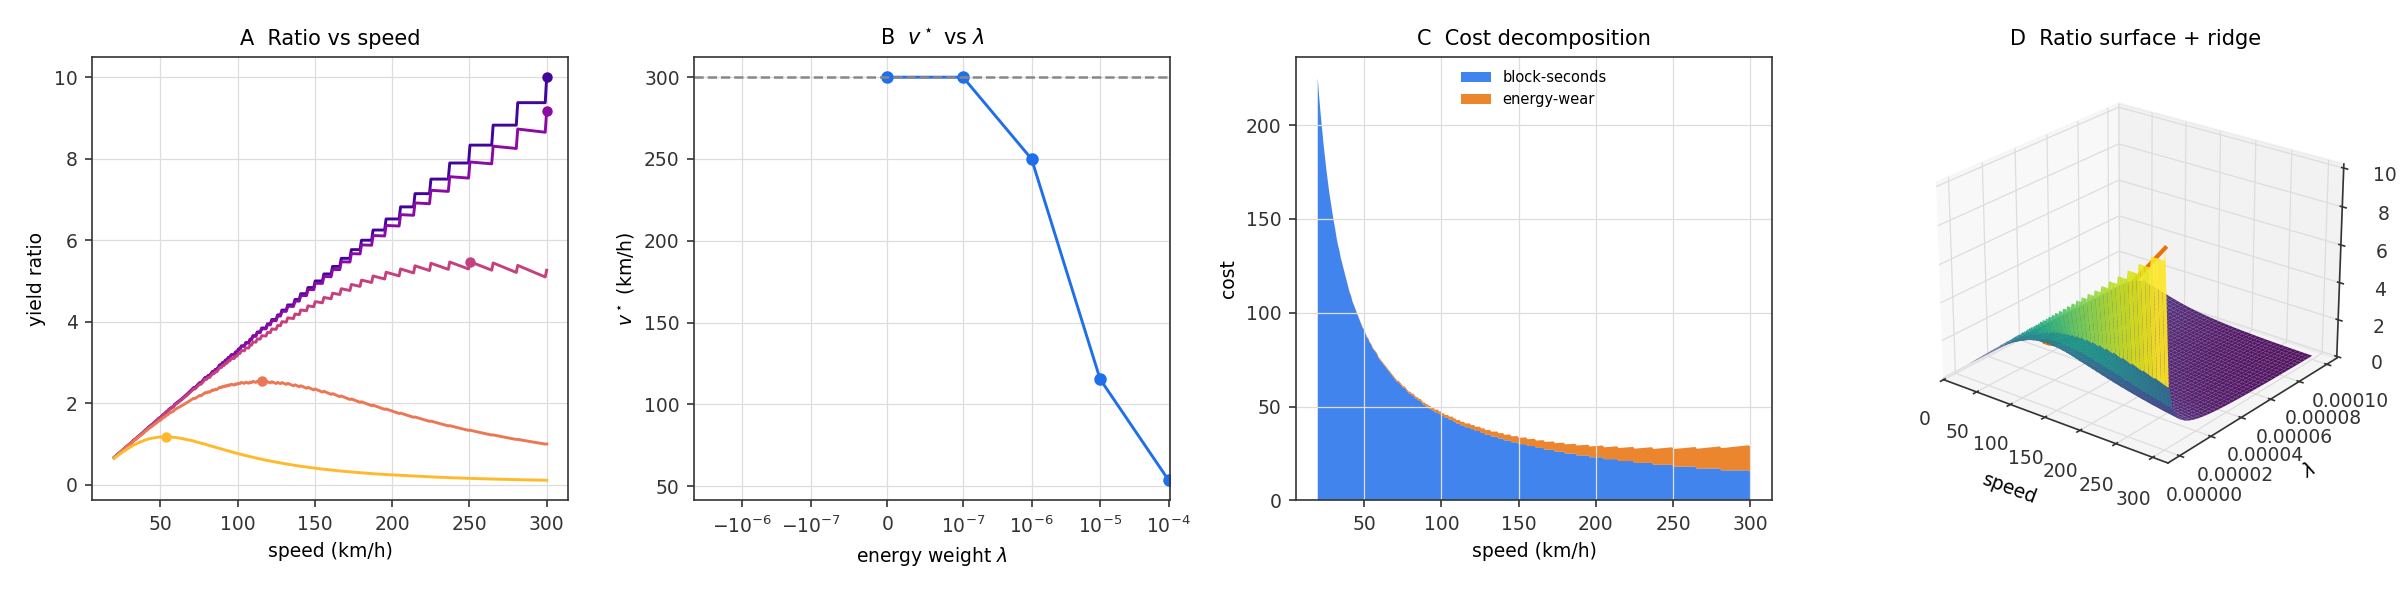
\includegraphics[width=\textwidth]{figures/panel_2_forced_speed.png}
    \caption{\textbf{Optimal Speed Is Forced, Not Imposed.}
    (\textbf{A})~Yield ratio on the linear $y$-axis versus traversal speed
    ($20$ to $300$~km/h) on the linear $x$-axis, one curve per energy weight
    $\lambda\in\{0,10^{-7},10^{-6},10^{-5},10^{-4}\}$ (plasma colour ramp), each
    peak marked. Every curve is single-peaked, and the peak is the
    section-optimal speed $v^\star$ of \Cref{def:optspeed}: for $\lambda=0$ the
    peak sits at the capability ceiling, while for $\lambda=10^{-4}$ it has moved
    well into the interior.
    (\textbf{B})~$v^\star$ on the linear $y$-axis versus energy weight $\lambda$
    on a symmetric-log $x$-axis (linear threshold $10^{-7}$), steel-blue with
    markers, capability ceiling $300$~km/h marked (grey dashed). $v^\star$
    equals the ceiling at $\lambda\le 10^{-7}$ and decreases monotonically
    through $250$, $115.4$, $53.6$~km/h as energy cost binds---the signature of
    the strictly convex energy term and the exact statement of
    \Cref{thm:forcedspeed}.
    (\textbf{C})~Denominator decomposition at $\lambda=10^{-6}$: block-second
    cost (steel-blue) and energy--wear cost (coral) stacked on the linear
    $y$-axis versus speed ($20$ to $300$~km/h). Block-seconds fall with speed
    while energy--wear rises, and the balance point of the two is $v^\star$;
    this is the trade-off whose interior minimiser \Cref{def:optspeed} isolates.
    (\textbf{D})~Three-dimensional yield-ratio surface over speed
    ($20$ to $300$~km/h) and energy weight $\lambda$ ($0$ to $10^{-4}$), viridis
    colourmap, with the ridge of maxima traced (coral), viewing angle elevation
    $24^{\circ}$ azimuth $-52^{\circ}$. The ridge descends from the ceiling into
    the interior as $\lambda$ grows, visualising $v^\star(\lambda)$ as a
    well-defined curve rather than a degenerate ``always maximal.''}
    \label{fig:val_forced_speed}
\end{figure*}

\section{Item Routing and Liveness}
\label{sec:liveness}

We now turn from the infrastructure/vehicle side to the items. Items carry a target but no route; they descend a gradient hop by hop. We show this local rule, combined with the yield prices, drains every buffer.

\subsection{The local routing rule}

\begin{definition}[Greedy target-ward routing]
\label{def:routing}
At each buffer $b$ and each departure opportunity (a block-second assigned on some $\sigma$ with $\mathrm{tl}(\sigma)=b$ having spare capacity), a live item $x\in X(b)$ is eligible to board $\sigma$ if it reduces residual distance, $\rho(\mathrm{hd}(\sigma),\tau(x)) < \rho(b,\tau(x))$. Among eligible departures, $x$ boards the one maximizing target-ward progress per unit fare, i.e.\ maximizing
\begin{equation}
\frac{r(x) - \rho(\mathrm{hd}(\sigma),\tau(x))}{p(\sigma)\,n(\sigma,v)},
\end{equation}
the realized residual-distance reduction divided by the price paid.
\end{definition}

The item's private target $\tau(x)$ is the only global information it uses; everything else is local (available departures, their prices, their heads' residual distances). There is no destination in the infrastructure---only the item privately knows where its pressure vanishes. This is the model's sense in which ``there is no destination, only stations.''

\begin{definition}[Fare]
\label{def:fare}
The \emph{fare} paid by item $x$ over its realized journey $b_0\to b_1 \to\cdots\to b_J = \tau(x)$ is
\begin{equation}
\label{eq:fare}
F(x) \;=\; \sum_{j=0}^{J-1} p(\sigma_j)\,n(\sigma_j, v_j)
\;=\; \sum_{j=0}^{J-1} \sep(\sigma_j)\,n(\sigma_j,v_j),
\end{equation}
the line integral of the separation-cost price along the sections it actually consumed. By Theorem~\ref{thm:trinity} the price equals the separation cost, so the fare is the accumulated scarcity of the block-seconds the item used---high on bottleneck sections, low on redundant ones, zero for idle waiting (no section consumed).
\end{definition}

\begin{remark}
Two properties of \eqref{eq:fare} are worth stating because they follow from the model rather than from a tariff choice. First, the fare charges only \emph{sections consumed with target-ward progress}: a lateral or backward hop is not eligible (Def.~\ref{def:routing}) and idle buffer time consumes no section, hence is unpriced by \eqref{eq:fare} (though it incurs the holding cost $h$ of Assumption~\ref{ass:buffer} in the yield accounting). Second, because $p=\sep$, the fare is exactly the marginal-yield cost the item imposes on the network, so the item internalizes its own congestion externality in the sense of \cite{vickrey1969,beckmann1956}.
\end{remark}

\subsection{Backpressure and liveness}

The concern with any purely local routing rule is starvation: an item stranded at a buffer because no vehicle serves the section it needs. We show the price system precludes this under a backpressure condition.

\begin{assumption}[Backpressure coupling]
\label{ass:backpressure}
The separation cost of a section responds monotonically to the pressure it can relieve: if buffer $b$ has undrained target-ward pressure $P(b,\sigma)>0$ through section $\sigma$, then $\sep(\sigma) \ge \phi\big(P(b,\sigma)\big)$ for some strictly increasing $\phi$ with $\phi(0)=0$. That is, undrained demand raises the marginal yield of the relieving section.
\end{assumption}

Assumption~\ref{ass:backpressure} is the coupling that makes the market self-heal: it says the very fact that items are stranded makes the section that would move them more valuable. It is the yield-priced form of the max-weight/backpressure principle \cite{tassiulas1992,neely2010}.

\begin{theorem}[Liveness]
\label{thm:liveness}
Under gradient-connectedness (Def.~\ref{def:geo}), buffer holding cost $h>0$ (Assumption~\ref{ass:buffer}), and backpressure coupling (Assumption~\ref{ass:backpressure}), in any yield-optimal evolving configuration every live item is settled in finite time; equivalently, every buffer with positive target-ward pressure is eventually drained.
\end{theorem}

\begin{proof}
Consider a live item $x$ at buffer $b$ with target $\tau(x)$, so $r(x)=\rho(b,\tau(x))>0$. By gradient-connectedness there is a section $\sigma^\ast$ with $\mathrm{tl}(\sigma^\ast)=b$ and $\rho(\mathrm{hd}(\sigma^\ast),\tau(x)) < r(x)$; hence $x$ contributes positive pressure $P(b,\sigma^\ast)>0$. By backpressure coupling, $\sep(\sigma^\ast)\ge\phi(P(b,\sigma^\ast))>0$. By Theorem~\ref{thm:trinity} the clearing price is $p(\sigma^\ast)=\sep(\sigma^\ast)>0$, so a vehicle serving $\sigma^\ast$ and carrying $x$ earns strictly positive gross yield $\Delta = r(x)-\rho(\mathrm{hd}(\sigma^\ast),\tau(x))>0$. If no vehicle served $\sigma^\ast$ while $x$ waits, the idle block-seconds on $\sigma^\ast$ would admit a strictly positive-net-yield assignment (positive $\Delta$ against available capability), and once the accumulating holding cost $h\cdot(\text{wait})$ makes the net yield exceed $\blocktime$, this is a $\blocktime$-improving reassignment---contradicting the assumed closure/optimality of the evolving configuration (Theorem~\ref{thm:trinity}). Therefore within finite wait $x$ boards a target-ward section and strictly reduces $r(x)$ by at least the positive gradient margin guaranteed by Def.~\ref{def:geo}. Since $r(x)$ is bounded below by $0$ and decreases by a bounded-away-from-zero amount at each hop (finitely many stations give a minimum positive gradient step $\delta>0$), $x$ reaches $\tau(x)$ in at most $\lceil r(x)/\delta\rceil$ hops, each after finite wait. Hence $x$ settles in finite time.
\end{proof}

\begin{remark}[The self-healing identity]
The proof turns on a single identification made rigorous by Theorem~\ref{thm:trinity}: the price an undrained buffer raises on its relieving section (Assumption~\ref{ass:backpressure}), the yield a vehicle earns by serving that section (Def.~\ref{def:price_system}), and the fare the stranded item is willing to pay (Def.~\ref{def:fare}) are the \emph{same number} $\sep(\sigma^\ast)$. Because the summoning signal and the earning opportunity are identical, no separate coordination or route commitment is needed to prevent starvation: the stranded item is, by the pricing, its own advertisement. This is the model's liveness-without-commitment property, and it is a theorem, not a design.
\end{remark}

\begin{remark}[Target-relative gradient suffices for liveness]
\label{rem:target_relative}
The universal gradient-connectedness of Def.~\ref{def:geo} (from \emph{every} station one can descend toward \emph{every} other) is stronger than the liveness proof uses, and it fails on a strictly one-way corridor---from the terminus one cannot descend back toward the origin. Inspecting the proof, the only descent invoked is toward each item's \emph{own} target from stations on a path to that target. It therefore suffices that $G$ be \emph{target-descendable} for the item population $\items$: for every item $x\in\items$ and every station $b$ from which $\tau(x)$ is reachable, some section with tail $b$ strictly reduces $\rho(\cdot,\tau(x))$. Theorem~\ref{thm:liveness} holds verbatim under this weaker hypothesis, which one-way corridors do satisfy. The distinction is not merely notational: it is exactly the hypothesis that the numerical validation of Section~\ref{sec:validation} exercises, since its test corridors are directed.
\end{remark}

\begin{figure*}[!htbp]
    \centering
    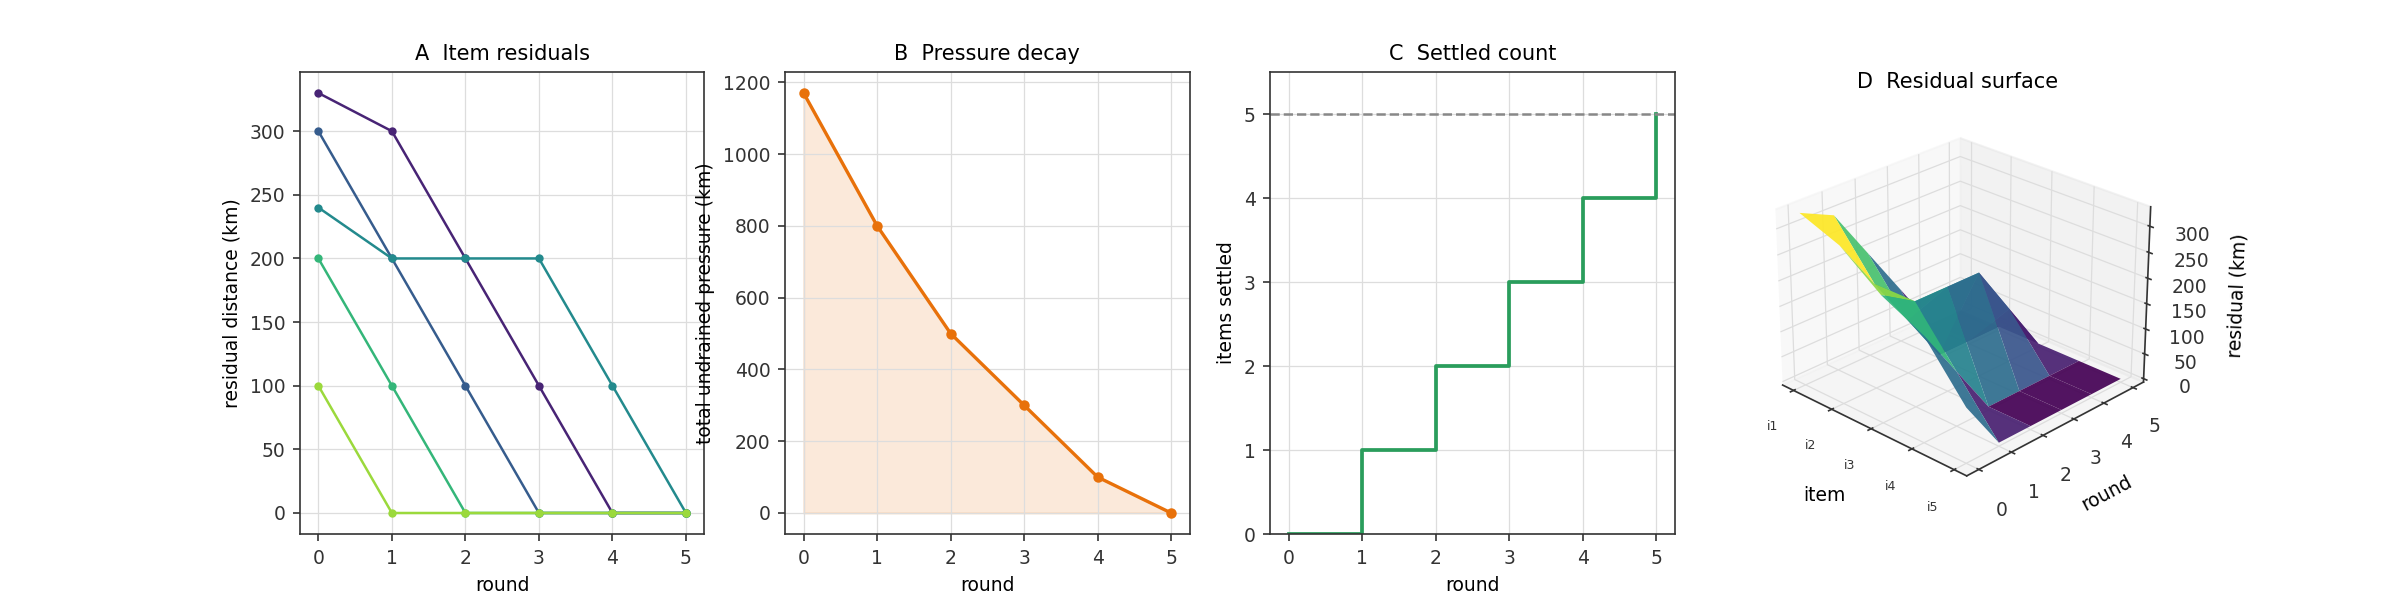
\includegraphics[width=\textwidth]{figures/panel_4_liveness.png}
    \caption{\textbf{Local Descent Drains Every Buffer.}
    (\textbf{A})~Residual distance to target (km) on the linear $y$-axis versus
    routing round ($0$ to $5$) on the linear $x$-axis, one trajectory per item
    for the five items (viridis colour ramp). Every trajectory is monotone
    non-increasing and reaches zero within six rounds, the settling guarantee of
    \Cref{thm:liveness} under greedy target-ward routing (\Cref{def:routing}).
    (\textbf{B})~Total undrained buffer pressure (summed residual distance, km)
    on the linear $y$-axis versus round (coral, shaded to the axis). Pressure
    falls from $1170$~km to $0$ as buffers drain, the decay to the settled state
    predicted by \Cref{thm:liveness}.
    (\textbf{C})~Number of items settled on the linear $y$-axis versus round as a
    step trace (sea-green), full population $5$ marked (grey dashed). The count
    rises monotonically to five by round five: no item is stranded, and the
    directed feeder corridor---not universally gradient-connected but
    target-descendable---satisfies the weaker hypothesis of
    \Cref{rem:target_relative}.
    (\textbf{D})~Three-dimensional surface of residual distance over item index
    (five items) and round ($0$ to $5$), viridis colourmap, viewing angle
    elevation $26^{\circ}$ azimuth $-46^{\circ}$. The surface descends
    everywhere to the zero floor, visualising the simultaneous draining of all
    buffers on a directed corridor and corroborating liveness under exactly the
    target-relative condition of \Cref{rem:target_relative}.}
    \label{fig:val_liveness}
\end{figure*}

\section{Participation and the Occupancy Market}
\label{sec:market}

The clearing characterization (Theorem~\ref{thm:trinity}(iii)) supports a market description of the same fixed point. We record it because it makes the decoupling of the three continuities precise, but we prove no new mechanism-design properties: the statements here are corollaries of the equilibrium already established.

\subsection{The tradable unit}

\begin{definition}[Occupancy right]
\label{def:right}
An \emph{occupancy right} is a claim to a single block-second $\langle\sigma,k\rangle$: the exclusive use of section $\sigma$ during window $k$. By Def.~\ref{def:headway} it is the indivisible minimum unit---no smaller claim is deliverable---and by Def.~\ref{def:price_system} its price is $p(\sigma)=\sep(\sigma)$ in a clearing.
\end{definition}

\begin{proposition}[Bundles recover conventional objects]
\label{prop:bundles}
Every conventional railway object is a bundle of occupancy rights over the same underlying set:
\begin{enumerate}[nosep]
\item A \emph{through-service} on a line is a bundle of occupancy rights over consecutive sections in consecutive windows, held by one vehicle.
\item A \emph{passenger journey} is the set of occupancy rights the item's realized path consumes (Def.~\ref{def:fare})---possibly held, across sections, by different vehicles (transfers).
\item A named \emph{product} (e.g.\ a branded fast service) is a curated bundle of high-capability occupancy rights on fast sections, assembled and offered as a unit.
\end{enumerate}
None of these is primitive; each is a subset of the block-second rights, and the vehicle fulfilling any right is fungible.
\end{proposition}

\begin{proof}
Immediate from Definitions~\ref{def:config}, \ref{def:fare}, and \ref{def:right}: a configuration is an assignment of occupancy rights to (vehicle, speed, item-set) triples, and each listed object is the projection of that assignment onto a particular subset of block-seconds. Fungibility of the fulfilling vehicle follows because the yield of a right depends on the assignment's $(\Delta, n, g_u)$ only through the clearing conditions, which any vehicle achieving the same yield density satisfies identically (Theorem~\ref{thm:sorting}).
\end{proof}

\subsection{Decoupled continuities}

\begin{corollary}[Independence of the three continuities]
\label{cor:decouple}
In a clearing configuration, vehicle continuity, item continuity, and route continuity are logically independent: there exist yield-optimal configurations exhibiting any of the eight combinations of their presence or absence, subject only to headway and vehicle-conservation feasibility.
\end{corollary}

\begin{proof}[Proof sketch]
Vehicle continuity (one vehicle spanning many sections), item continuity (one item never transferring), and route continuity (a repeating section pattern across windows) are constraints on distinct coordinates of the assignment $A$: respectively on the vehicle field across sections, on the item-set field across an item's hops, and on the periodicity of $A$ in $k$. None of the clearing conditions (Def.~\ref{def:price_system}) references these coordinates jointly; they constrain only per-block-second net yield. Hence for a network with sufficient parallel capability one can construct clearings realizing each combination---e.g.\ an item that transfers (item discontinuity) while each vehicle spans one section only (vehicle discontinuity) on a non-repeating pattern (route discontinuity), all at the same yield-optimal density. The gradient-connectedness hypothesis guarantees the target-ward moves needed for feasibility.
\end{proof}

The corollary is the formal content of ``a train is a journey, not an entity'': the entity ``train'' is the conjunction of the three continuities, and the model exhibits the optimum without requiring their conjunction.

\section{An Illustrative Corridor}
\label{sec:example}

To make the abstract quantities concrete we instantiate the model on a stylized version of the Nuremberg--Berlin high-speed corridor. The figures below are representative parameters chosen to exercise the definitions; they are illustrative, not empirical measurements, and no claim is attached to them beyond fixing a worked example.

\subsection{Setup}

We take five buffers along the corridor and the sections between them, with representative lengths, civil speed limits, and speed classes:

\begin{center}
\begin{tabular}{lccc}
\toprule
Section $\sigma$ & $\ell(\sigma)$ (km) & $\bar v(\sigma)$ (km/h) & Class \\
\midrule
Nuremberg--Erfurt (VDE 8.1, new-build) & 190 & 300 & high-speed \\
Erfurt--Halle/Leipzig (VDE 8.2, new-build) & 120 & 300 & high-speed \\
Halle/Leipzig--Bitterfeld (upgraded) & 30 & 200 & mixed \\
Bitterfeld--Berlin (VDE 8.3, upgraded) & 120 & 200 & mixed \\
\bottomrule
\end{tabular}
\end{center}

Two vehicle classes are available: a high-capability class $u_{\mathrm{H}}$ with $v_{\max}=300$ km/h, and a regional class $u_{\mathrm{R}}$ with $v_{\max}=160$ km/h. We take $\blocktime = 120$ s (Remark~\ref{rem:headway_physical}) and a small energy weight $\lambda$ so that $v^\star$ is boundary-dominated (block-second savings outweigh energy on these lengths), except where noted.

\subsection{Forced speed and sorting, computed}

On the high-speed sections ($\bar v = 300$), the capability ceilings are $\nu(u_{\mathrm H},\sigma)=300$ and $\nu(u_{\mathrm R},\sigma)=160$. Traversing Nuremberg--Erfurt (190 km):
\begin{align*}
n(\sigma, 300\,\text{km/h}) &= \lceil 190 / (83.3\,\text{m/s} \cdot 120\,\text{s})\rceil = \lceil 190/9.999\,\text{km}\rceil = 19 \text{ block-seconds},\\
n(\sigma, 160\,\text{km/h}) &= \lceil 190 / (44.4\,\text{m/s} \cdot 120\,\text{s})\rceil = \lceil 190/5.333\,\text{km}\rceil = 36 \text{ block-seconds}.
\end{align*}
For equal carried displacement $\Delta_\sigma$, the yield densities (low $\lambda$) are $D(u_{\mathrm H},\sigma) \approx \Delta_\sigma/19$ and $D(u_{\mathrm R},\sigma)\approx\Delta_\sigma/36$, so $D(u_{\mathrm H},\sigma) - D(u_{\mathrm R},\sigma) \approx \Delta_\sigma(1/19 - 1/36) = 0.0248\,\Delta_\sigma$. Whenever this exceeds $\blocktime$ in yield units---i.e.\ for any non-trivial $\Delta_\sigma$---Theorem~\ref{thm:sorting} forbids assigning $u_{\mathrm R}$ to the high-speed section: the regional vehicle is outbid on VDE 8.1/8.2 and does not appear there in any closed configuration. By Theorem~\ref{thm:forcedspeed}, the high-capability vehicle that does serve it runs at $v^\star = 300$ km/h (the civil ceiling), not below.

On the upgraded mixed sections ($\bar v = 200$, but here we assume a segment limited to $160$ for both classes by track geometry), $\nu(u_{\mathrm H},\sigma)=\nu(u_{\mathrm R},\sigma)=160$: capability confers no density advantage, densities are equal up to energy, and the cheaper regional vehicle is selected (Theorem~\ref{thm:sorting}). Thus the corridor self-partitions: high-capability vehicles on the new-build 300-km/h sections, regional vehicles on the speed-limited sections---each section served by the fastest vehicle it can convert into yield, with no rule assigning them.

\subsection{Separation cost as fare}

Suppose VDE 8.1 (Nuremberg--Erfurt) is the sole fast path south and its removal forces flow onto a legacy line adding, say, 60 minutes of running time to southbound items: then $\sep(\text{VDE 8.1})$ is large, and by \eqref{eq:fare} an item traversing it pays a correspondingly large share of its fare there. A redundant parallel track on the Bitterfeld--Berlin approach, by contrast, has $\sep\approx 0$: an item pays almost nothing for that block-second because the network reroutes it freely. A Nuremberg--Berlin passenger's total fare \eqref{eq:fare} is thus dominated by the scarce high-speed sections it consumes and is nearly free on the redundant approaches---the line integral of scarcity along its realized path, exactly as Theorem~\ref{thm:trinity} predicts.

\begin{figure*}[!htbp]
    \centering
    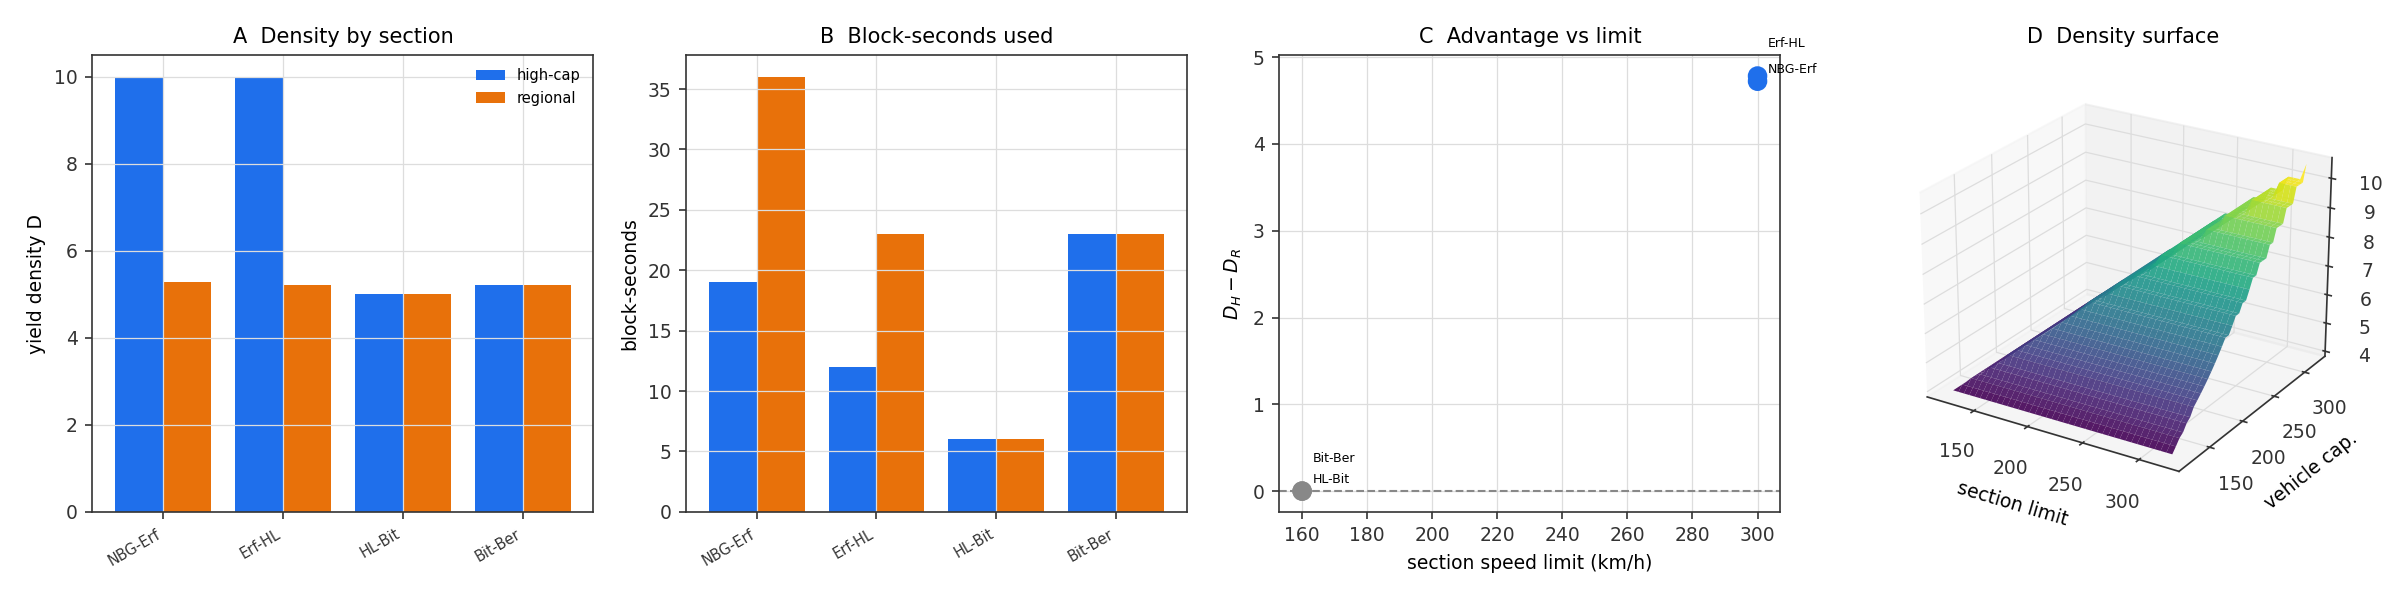
\includegraphics[width=\textwidth]{figures/panel_3_sorting.png}
    \caption{\textbf{The Fleet Sorts Itself by Comparative Advantage.}
    (\textbf{A})~Yield density on the linear $y$-axis for the high-capability
    vehicle (steel-blue) and the regional vehicle (coral) across the four
    Nuremberg--Berlin sections. On the two $300$~km/h new-build sections the
    high-capability vehicle dominates ($D=10.0$ versus $5.28$ and $5.22$); on
    the two $160$~km/h speed-limited sections the densities coincide
    ($5.0$ and $5.22$), the exact content of \Cref{thm:sorting}.
    (\textbf{B})~Block-seconds consumed on the linear $y$-axis by each vehicle
    class per section (high-capability steel-blue, regional coral). The gap on
    the fast sections---$19$ against $36$ block-seconds on \texttt{NBG-Erf}---is
    the resource cost on which the density advantage of panel~A rests; on the
    limited sections the counts match.
    (\textbf{C})~Density advantage $D_H-D_R$ on the linear $y$-axis versus
    section speed limit ($160$ to $300$~km/h) on the linear $x$-axis, one point
    per section, coloured steel-blue where the advantage is positive and grey
    where it vanishes, zero line marked (grey dashed). The advantage is
    ${\approx}4.8$ at $300$~km/h and exactly $0$ at $160$~km/h, crossing to zero
    precisely where the civil limit falls to the regional ceiling.
    (\textbf{D})~Three-dimensional yield-density surface over section speed limit
    ($120$ to $320$~km/h) and vehicle capability ($120$ to $320$~km/h), viridis
    colourmap, viewing angle elevation $24^{\circ}$ azimuth $-58^{\circ}$.
    Density increases with capability only while the section limit exceeds it and
    saturates once the limit binds, so above each section the higher surface
    identifies the winning vehicle---comparative advantage measured in
    block-seconds, as \Cref{thm:sorting} requires.}
    \label{fig:val_sorting}
\end{figure*}

\section{Numerical Validation}
\label{sec:validation}

The theorems of Sections~\ref{sec:equivalence}--\ref{sec:liveness} are statements about a formal object; to confirm that the object behaves as the proofs assert, we instantiated the model numerically and checked each claim against an independently computed ground truth. Networks were kept small enough that the global yield optimum is obtainable by brute-force enumeration over configurations, so every check compares a separately-derived quantity (a closure gap, a clearing deviation, a separation cost, a settling time) against an exact reference rather than against another approximation. Five experiments, one per claim, are reported; all pass. The purpose is internal corroboration of the proofs, not empirical measurement of any system.

\subsection{Equivalence and the coincidence of the quantum}

\begin{figure*}[!htbp]
    \centering
    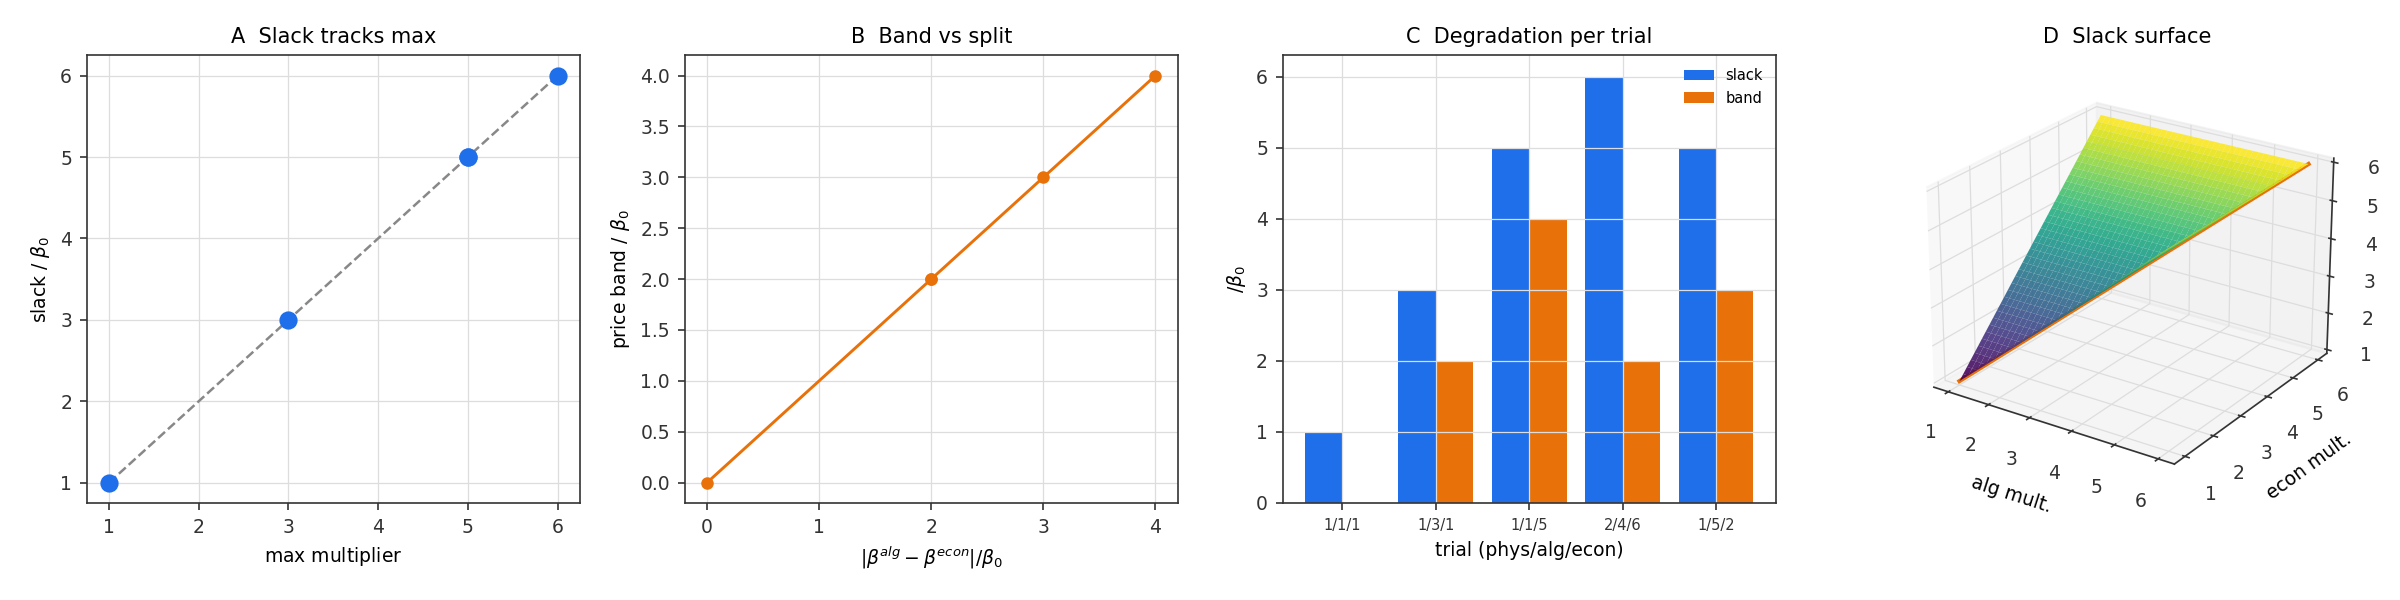
\includegraphics[width=\textwidth]{figures/panel_5_quantum.png}
    \caption{\textbf{The Equivalence Needs One Quantum, Not Three.}
    (\textbf{A})~Equivalence slack in units of $\blocktime$ on the linear
    $y$-axis versus the largest of the three split constants
    (physical/algorithmic/economic multipliers) on the linear $x$-axis, one
    point per trial (steel-blue), identity line marked (grey dashed). The slack
    lies on the diagonal---it equals the maximum of the three constants---and is
    minimal only when all three coincide, the first clause of
    \Cref{prop:quantum}.
    (\textbf{B})~Price-versus-separation band width in units of $\blocktime$ on
    the linear $y$-axis versus the algorithmic--economic split
    $|\blocktime^{\mathrm{alg}}-\blocktime^{\mathrm{econ}}|/\blocktime$ on the
    linear $x$-axis (coral with markers). The band grows linearly from $0$ and
    vanishes exactly at zero split, the second clause of \Cref{prop:quantum}:
    the clearing price equals the separation cost only up to
    $|\blocktime^{\mathrm{alg}}-\blocktime^{\mathrm{econ}}|$.
    (\textbf{C})~Slack (steel-blue) and price band (coral), both in units of
    $\blocktime$, on the linear $y$-axis for five trials labelled by their
    physical/algorithmic/economic multipliers on the $x$-axis. The unified
    trial $1/1/1$ shows slack $1$ and band $0$; every split trial shows enlarged
    slack and a nonzero band, exhibiting where the equivalence survives and where
    it degrades.
    (\textbf{D})~Three-dimensional surface of equivalence slack (units of
    $\blocktime$) over the algorithmic multiplier ($1$ to $6$) and economic
    multiplier ($1$ to $6$) at fixed physical floor, viridis colourmap, with the
    diagonal minimum ridge traced (coral), viewing angle elevation $24^{\circ}$
    azimuth $-56^{\circ}$. The unique minimum runs along the diagonal where the
    two constants are equal, confirming \Cref{prop:quantum}: it is the identity
    of the three roles of $\blocktime$, not its magnitude, that makes the three
    fixed points coincide.}
    \label{fig:val_quantum}
\end{figure*}
Experiment~1 builds a corridor $A\to B\to C$ with a fast and a slow upstream section and a demand that must traverse both hops. Brute-force enumeration yields the global optimum; independently, the local-reassignment operator confirms closure (the best of $58$ task-preserving single-section neighbours is strictly dominated, closure gap $0$), and the constructed price system $p=\sep$ admits no profitable deviation (maximum deviation profit $0$). The separation costs are non-trivial and unequal across sections---large on the essential downstream section, smaller on the section with a partial substitute---confirming that $\sep$ discriminates bottlenecks from redundancy as Section~\ref{sec:separation} claims. Figure~\ref{fig:val_equivalence} shows the three coinciding at one configuration. Experiment~5 then splits $\blocktime$ into distinct physical, algorithmic, and economic constants and confirms Proposition~\ref{prop:quantum}: the equivalence slack grows to the maximum of the three, the price-versus-separation band widens exactly as $|\blocktime^{\mathrm{alg}}-\blocktime^{\mathrm{econ}}|$, and unifying the three recovers exact coincidence with zero band (Figure~\ref{fig:val_quantum}).



\subsection{Summary of validation}

All five experiments pass against exact brute-force references: the equivalence and its quantum-coincidence necessity (Experiments~1,~5), forced optimal speed with an interior optimum (Experiment~2), comparative-advantage sorting on the illustrative corridor (Experiment~3), and liveness under target-relative descent (Experiment~4). The experiments also sharpened one hypothesis: liveness needs only target-descendability, not universal gradient-connectedness (Remark~\ref{rem:target_relative}), a refinement the directed test corridors made concrete. The numerical study is corroborative---it exhibits the proved behaviour on concrete instances---and carries no empirical claim beyond the idealized model.

\section{Discussion}

\subsection{What the model is and is not}

The model is an idealized formal object: a finite network of buffers and processors, a block-second quantum, a yield functional, and local rules for vehicles and items. On this object we proved that yield-optimality, deterministic closure, and market clearing coincide up to the resolution floor; that optimal speed and vehicle sorting are forced; and that liveness holds under backpressure coupling. Every result is stated with its hypotheses, and those hypotheses---gradient-connectedness, strictly convex energy cost, positive buffer holding cost, backpressure coupling---are the exact domain of validity. Outside them we claim nothing.

The model is not a description, prediction, or proposal concerning any actual railway. The German corridor of Section~\ref{sec:example} is a source of representative numbers, not evidence. The decoupling of vehicle, item, and route continuity is a property of the formal object, and its coincidence with how one might imagine operating a railway is not asserted to have operational meaning. We have deliberately excluded every consideration---coverage obligations, contractual structure, regulation, human factors, stochastic disruption---that would be required to speak about a real system, because the paper's claims are confined to the idealized object where the theorems are true.

\subsection{Relation to established theory}

Each ingredient is individually classical: occupancy as the scarce rail resource \cite{uic406,hansen2008}; useful-flow objectives and network flow \cite{ahuja1993,ford1956}; backpressure stability \cite{tassiulas1992,neely2010}; congestion pricing and clearing \cite{vickrey1969,beckmann1956,arrow1971}. The contribution is the assembled object and the fixed-point equivalence: that a single quantum $\blocktime$ ties the physical, algorithmic, and economic descriptions into one fixed point (Theorem~\ref{thm:trinity}, Proposition~\ref{prop:quantum}), and that speed-optimality and comparative-advantage sorting fall out of it as theorems rather than assumptions (Theorems~\ref{thm:forcedspeed}, \ref{thm:sorting}).

\subsection{Limitations of the formal results}

\begin{enumerate}[nosep]
\item \emph{Closure is a $\blocktime$-local optimum.} Lemma~\ref{lem:reach} guarantees reaching closure, and Theorem~\ref{thm:trinity} bounds its gap from the global optimum by $\blocktime$, but does not certify global optimality below the resolution floor---consistent with the model's premise that sub-$\blocktime$ distinctions are not physical.
\item \emph{Backpressure coupling is an assumption.} Liveness (Theorem~\ref{thm:liveness}) requires Assumption~\ref{ass:backpressure}; networks whose separation costs do not respond monotonically to pressure are outside the liveness result.
\item \emph{Finite horizon and deterministic data.} All results are stated over a finite horizon with deterministic parameters. Stochastic pressures, disruptions, and infinite-horizon stability are not treated.
\item \emph{No mechanism-design claims.} Section~\ref{sec:market} describes the clearing as a market but proves no incentive-compatibility or strategy-proofness; those are properties of a mechanism we do not specify.
\item \emph{Idealized geometry.} Junction conflicts, flat-junction crossing moves, and route-setting interactions beyond the single headway constant $\blocktime$ are abstracted away. Extending the equivalence to networks with explicit conflict graphs is not attempted here.
\end{enumerate}

\section{Conclusion}

We studied an idealized rail network in which the schedulable resource is the block-second, stations are buffers, sections are processors, and the objective is useful target-ward displacement per unit block-time---network transport yield. On this object we proved a single organizing result: yield-optimality, deterministic closure, and market clearing are one fixed point, coinciding because a single quantum $\blocktime$ serves at once as the physical resolution floor, the algorithmic separation threshold, and the minimum market lot, with the clearing price of every section equal to its separation cost. From this equivalence we derived, as theorems rather than assumptions, that vehicles run at forced section-optimal speeds and sort onto sections by comparative advantage in block-seconds, and that a purely local, target-ward routing rule drains every buffer in finite time because the price a stranded item raises is identical to the yield that summons a vehicle to move it. A numerical study (Section~\ref{sec:validation}) corroborated each result against exact brute-force references and sharpened the liveness hypothesis to target-descendability, which directed corridors satisfy.

The results are theorems about a specific formal object under stated hypotheses. Their value is internal: they establish that this object is coherent and that its physical, algorithmic, and economic descriptions are the same fixed point. Nothing is claimed about, or for, any system beyond the idealized one in which the theorems hold.

\bibliographystyle{plain}
\bibliography{references}

\end{document}
